%TODO mettre les nuémros des questions
%TODO ref entre sections

\documentclass[10pt,a4paper]{article}
\usepackage[utf8]{inputenc}
\usepackage[french]{babel}
\usepackage[T1]{fontenc}
\usepackage{amsmath}
\usepackage{amsfonts}
\usepackage{amssymb}
\usepackage{graphicx}
\usepackage[colorlinks = true,
            linkcolor = blue,
            urlcolor  = blue,
            citecolor = blue,
            anchorcolor = blue]{hyperref}
\title{Apprentissage profond par renforcement \\ Compte-rendu de TP}
\author{Nelly Barret et Juliette Reisser}

% code
\usepackage{listings}
\usepackage{xcolor}
\definecolor{codegreen}{rgb}{0,0.6,0}
\definecolor{codegray}{rgb}{0.5,0.5,0.5}
\definecolor{codepurple}{rgb}{0.58,0,0.82}
\definecolor{backcolour}{rgb}{0.95,0.95,0.92}
\lstdefinestyle{mystyle}{
    backgroundcolor=\color{backcolour},   
    commentstyle=\color{codegreen},
    keywordstyle=\color{magenta},
    numberstyle=\tiny\color{codegray},
    stringstyle=\color{codepurple},
    basicstyle=\ttfamily\footnotesize,
    breakatwhitespace=false,         
    breaklines=true,                 
    captionpos=b,                    
    keepspaces=true,                 
    numbers=left,                    
    numbersep=5pt,                  
    showspaces=false,                
    showstringspaces=false,
    showtabs=false,                  
    tabsize=2
}
\lstset{style=mystyle}

% subsubsubsection
\usepackage{titlesec}

\setcounter{secnumdepth}{4}

\titleformat{\paragraph}
{\normalfont\normalsize\bfseries}{\theparagraph}{1em}{}
\titlespacing*{\paragraph}
{0pt}{3.25ex plus 1ex minus .2ex}{1.5ex plus .2ex}


\begin{document}
\maketitle

\section{Préliminaires} \label{prelim}
Notre TP se trouve à l'adresse suivante : \href{https://github.com/NellyBarret/IA5-TP-APR}{https://github.com/NellyBarret/IA5-TP-APR}

Nous avons principalement utilisé les libraires suivantes :
\begin{itemize}
	\item \href{https://gym.openai.com/}{Gym} pour les environnements d'apprentissage
	\item \href{https://keras.io/}{Keras} (de Tensorflow) pour les modèles de réseaux neuronaux
	\item \href{https://numpy.org/}{Numpy} pour les calculs
	\item \href{https://matplotlib.org/index.html}{Matplotlib} pour les tracés de courbe
\end{itemize}

Nous allons d'abord définir quelques variables communes aux différentes implémentations. Ces variables font partie de la logique même utilisée par Gym.

Nous avons accès à deux variables importantes quant à la définition de l'environnement :
\begin{itemize}
	\item L'\textbf{espace des actions} (\lstinline{env.action_space}) qui définit les actions possibles pour l'agent. Chaque action est un entier, e.g. 0 pour aller à gauche, 1 pour aller à droite.
	\item L'\textbf{espace des observations}, ou \textbf{espace d'états}, (\lstinline{env.observation_space}) qui définit un tableau représentant les métriques importantes de l'environnement, e.g. la position d'un élément, les frames d'un jeu...
\end{itemize}

Nous avons aussi 3 variables importantes quant à l'exécution d'actions sur l'environnement :
\begin{itemize}
	\item \lstinline{next_state} qui définit le \textbf{nouvel état} (après exécution de l'action sur l'environnement)
	\item \lstinline{reward} qui représente la \textbf{récompense} gagnée par l'agent après exécution de l'action sur l'environnement
	\item \lstinline{done} qui est un booléen indiquant si l'épisode courant est fini, e.g. le bâton est tombé
\end{itemize}

Enfin, nous avons deux méthodes importantes quant à la communication environnement/agent :
\begin{itemize}
	\item \lstinline{act()} qui retourne l'\textbf{action} choisie par l'agent. C'est dans cette fonction que nous implémenterons les \textbf{politiques} (de sélection d'action), i.e. aléatoire, $\epsilon$-greedy et Boltzmann. 
	\item \lstinline{step(action)} qui exécute une action sur l'environnement et retourne les 3 variables expliquées ci-dessus. 
\end{itemize}

Maintenant que nous avons définit les variables importantes, nous allons définir le fonctionnement général des agents.

\begin{lstlisting}[language=Python, caption=Pseudo-code du fonctionnement de l'agent dans son environnement]
env = gym.make("nom-environnement")
agent = Agent()

Pour chaque episode dans (0, nb_max_epsiodes), Faire
    Tant que True, Faire:
        action = agent.act()
        next_state, reward, done, info = env.step(action)
        Si done == True, Faire:
            break
\end{lstlisting}

Dans un premier temps il est important de créer l'environnement voulu dans la variable \lstinline{env} et de créer un agent. C'est cet agent que nous allons entraîner dans l'environnement.
Le principe de l'entraînement de l'agent est le suivant : l'agent va interagir avec l'environnement pendant \lstinline{nb_max_epsiodes} épisodes. Un épisode correspond à toutes les actions que l'agent va pouvoir faire jusqu'à ce qu'une condition ne soit plus respectée (e.g. le bâton est tombé). Un épisode est donc une boucle qui se termine grâce à une condition, ici c'est \lstinline{done}. Durant cette boucle, l'agent choisit une nouvelle action à faire grâce à sa fonction \lstinline{act()} puis l'exécute d'ans l'environnement avec la fonction \lstinline{step(action)}. Pour résumer, un épisode est défini par la boucle \lstinline{Tant que} et l'agent s'entraîne pendant \lstinline{nb_max_episodes} épisodes.


\section{Agent aléatoire sur Cartpole}

Fichier correspondant : \href{https://github.com/NellyBarret/IA5-TP-APR/blob/master/randomCartPole.py}{randomCartpole.py}

\subsection{Définitions et fonctionnalités}

\subsubsection{Définition de l'environnement}

Dans l'environnement CartPole (variable \lstinline{env}), nous avons un bâton posé en équilibre sur un élément que l'on peut faire bouger à gauche ou à droite pour rééquilibrer le bâton. L'objectif principal pour l'agent est de maintenir le bâton assez vertical pour que celui-ci ne tombe pas et/ou ne sorte pas de l'environnement.

Nous allons maintenant spécifier les variables que nous avons défini en section \ref{prelim}.
\begin{itemize}
	\item L'espace des actions est de taille 2 car l'agent peut faire bouger l'élément à gauche (action 0) ou à droite (action 1)
	\item L'espace des états est de taille 4 car il est défini comme suit : [position de l'élément, vitesse de l'élément, angle du bâton, taux de rotation du bâton]
	\item La méthode \lstinline{act()} implémente une politique aléatoire (c.f. section \ref{defAgentRand})
\end{itemize}

\subsubsection{Définition de l'agent} \label{defAgentRand}

L'agent aléatoire suit une politique aléatoire pour choisir l'action qu'il va exécuter dans l'environnement. Il les choisit parmi ses actions possibles (disponibles dans \lstinline{env.action_space}). Il n'a pas de mémoire de ses précédentes expériences, ne prend pas en compte les gains futurs, ... . En somme, il exécute simplement des actions choisies aléatoirement.

\begin{lstlisting}[language=Python, caption=Programme principal de l'agent aléatoire]
env = gym.make("CartPole-v1")  # (1)
agent = RandomAgent(env.action_space)  # (1)
nb_episodes = 1000 # (2)
liste_rewards = [] # (3)
for i in range(nb_episodes): 
    total_reward = 0
    env.reset()
    while True: # (4)
        action = agent.act()
        _, reward, done, _ = env.step(action)
        total_reward += reward
        if done:
            break
        liste_rewards.append(total_reward) # (3)
evolution_rewards(liste_rewards)  # (3)
print("Meilleure recompense obtenue", max(liste_rewards), "lors de l'episode", liste_rewards.index(max(liste_rewards))) # (3)
env.close()

\end{lstlisting}

Le code ci-dessus montre l'instanciation du pseudo-code de l'entraînement d'un agent (en section \ref{prelim}).
\begin{lstlisting}[language=Python]
# (1)
\end{lstlisting}
Nous créons un environnement Gym avec comme paramètre le nom de l'environnement à créer (ici, \lstinline{"CartPole-v1"}). Nous créons ensuite notre agent aléatoire. Comme vu précédemment, celui-ci redéfinit la méthode \lstinline{act()}.

\begin{lstlisting}[language=Python]
# (2)
\end{lstlisting}
Nous devons ensuite choisir le nombre d'épisode sur lequel l'agent va s'entraîner. Comme l'agent a une politique aléatoire, le nombre d'épisode n'est pas un facteur influent sur les performances de l'agent puisque celui-ci exécute toujours des actions choisies aléatoirement. Nous prendrons comme paramètre 1000, ce qui permet de vérifier que l'agent interagisse correctement avec l'environnement sans pour autant que cela n'augmente (trop) le taux d'exécution.

\begin{lstlisting}[language=Python]
# (3)
\end{lstlisting}
Cette partie traite de l'évolution de la somme des récompenses perçues par l'agent. Pour chaque épisode nous ajoutons la récompense obtenue pour l'action choisie ce qui permet d'avoir une récompense \og globale \fg{}  par épisode. La fonction \lstinline{evolution_rewards} permet de tracer la courbe correspondant à ces récompenses par épisode.

Nous avons aussi récupéré la meilleure somme de récompense obtenue ainsi que le numéro de l'épisode où elle a été obtenue (ligne 16).

\begin{lstlisting}[language=Python]
# (4)
\end{lstlisting}
Dans cette partie là du code, nous rentrons dans un épisode. Dans cet épisode, nous devrons choisir une action puis l'exécuter dans l'environnement. La première étape est faite par la méthode \lstinline{act()}. Comme l'agent suit une politique aléatoire celle-ci retourne simplement une action parmi celles de l'espace d'actions de l'agent. Cela se traduit par le code ci-dessous :

\begin{lstlisting}[language=Python, caption=Implémentation de l'agent aléatoire]
class RandomAgent:
    """
    Agent qui choisit des actions de maniere aleatoire
    """
    def __init__(self, action_space):
        """
        Initialisation generale
        """
        self.action_space = action_space

    def act(self):
        """
        Choisit une action aleatoirement parmi l'espace d'actions
        """
        return self.action_space.sample()
\end{lstlisting}
Après avoir choisi une action, l'agent l'exécute dans l'environnement, ce qui lui permettra d'obtenir une récompense (ajoutée à la somme des récompenses de l'épisode en cours) et le booléen \lstinline{done}. Si ce booléen s'évalue à vrai, l'épisode se termine et le suivant commence. Sinon l'épisode continue et l'agent choisit une nouvelle action.

\subsection{Analyse de performances}

Pour évaluer notre agent aléatoire, nous avons réalisé un graphique traçant la somme des récompenses obtenues pour chaque épisode.

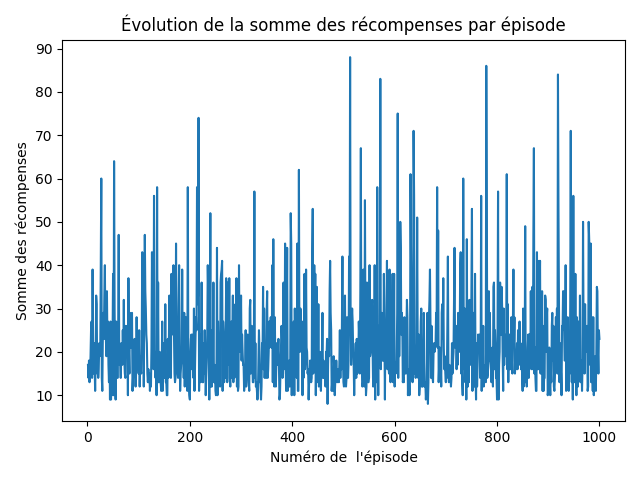
\includegraphics[scale=0.5]{evolution_recompenses_random.png} 

Nous pouvons observer qu'il n'y a pas de tendance particulière. Cela semble cohérent avec le fait que l'agent n'a aucun moyen d'apprendre de ses erreurs (pas de mémoire ni de rétro-propagation) et qu'il ne choisisse pas les meilleures actions (politique aléatoire).

\subsection{Experience replay}

Fichier correspondant : \href{https://github.com/NellyBarret/IA5-TP-APR/blob/master/ExperienceReplayAgent.py}{ExperienceReplayAgent.py}

Cet agent choisit aléatoirement ses actions et implémente une mémoire ce qui lui permettra par la suite d'apprendre par rapport à ses expériences passées.

\subsubsection{Définition de la mémoire}

\begin{lstlisting}[language=Python, caption=Implémentation de la mémoire d'un agent]
class Memory:
    """
    Classe representant la memoire de l'agent
    """
    def __init__(self, max_size, batch_size):
        """
        Initialise la memoire de l'agent
        @param max_size: taille maximale de la memoire
        @param batch_size: taille du batch genere
        """
        self.max_size = max_size
        self.memory = [[] for _ in range(self.max_size)]
        self.position = 0
        self.batch_size = batch_size

    def add(self, state, action, reward, next_state, done):
        """
        Ajoute une experience a la memoire de l'agent
        @param state: etat courant de l'agent
        @param action: action choisie par l'agent
        @param reward: recompense gagnee
        @param next_state: etat d'arrivee (apres action)
        @param done: True si l'experience est finie
        """
        self.memory[self.position] = [state, action, reward, next_state, done]
        self.position = (self.position + 1) % self.max_size

    def sample(self):
        """
        Construit un batch aleatoire sur la memoire de l'agent
        :return: le batch d'experiences
        """
        if self.__len__() < self.batch_size:
            return None
        else:
            batch = random.sample(self.memory, self.batch_size)
            return batch

    def __len__(self):
        """
        Retourne le nombre d'elements (non nuls) dans la memoire
        :return: le nombre d'elements dans la memoire
        """
        return sum(len(item) > 0 for item in self.memory)
\end{lstlisting}

Cette classe définit la mémoire de l'agent. Elle stocke les expérience que l'agent a avec l'environnement. La mémoire est donc modélisée par une liste d'expériences. Chaque expérience est une liste de 5 éléments : l'état courant de l'agent (variable \lstinline{state}), l'action choisie par l'agent (variable \lstinline{action}), la récompense obtenue pour cette action (variable \lstinline{reward}), l'état dans lequel va arriver l'agent après exécution de l'action (variable \lstinline{next_state}) et la variable \lstinline{done} qui indique si l'agent a terminé l'épisode ou non. 

$$
expe_i = [state_i, action_i, reward_i, nextstate_i, done_i]
$$

Cette mémoire a un nombre maximal d'éléments, donc quand un nouvel élément est inséré et qu'il n'y a plus de place, ce nouvel élément remplace le plus ancien. Elle est donc composée comme suit : 

$$
memory = \bigcup\limits_{i=1}^{max\_size} expe_{i} = 
\begin{bmatrix}
[state_1, action_1, reward_1, nextstate_1, done_1] \\
... \\
[state_n, action_n, reward_n, nextstate_n, done_n]
\end{bmatrix}
$$

De plus, nous avons deux fonctions pour interagir avec la mémoire :
\begin{itemize}
	\item \textit{L'ajout d'une nouvelle expérience} via la fonction \lstinline{add(...)} : cela ajoute à la mémoire de l'agent ce qu'il vient d'expérimenter dans l'environnement. Ce processus lui permettra par la suite d'apprendre de ses expériences passées.
	\item \textit{La création d'un batch} via la fonction \lstinline{sample()}: cette fonctionnalité crée un batch d'expériences en choisissant des éléments de manière aléatoire dans la mémoire.
\end{itemize}

Enfin, deux conditions sont à respecter :
\begin{enumerate}
	\item Le dépassement de la taille maximale doit être prévu. Il est prévu par le modulo utilisé pour la position de la nouvelle expérience à insérer. En effet, quand le buffer arrive à sa capacité, le modulo repart à 0, ce qui permet de remplacer les plus anciennes expériences par les nouvelles.
	\item La mémoire est indépendante de l’environnement, et donc de l’espace d’action et d’état. Cette condition est respectée du fait d'insérer au fur et à mesure dans la mémoire et de n'avoir qu'une taille maximale comme condition.
\end{enumerate}

\subsubsection{Définition de l'agent}

\begin{lstlisting}[language=Python, caption=Implémentation de l'agent utilisant son expérience]
class ExperienceReplayAgent:
    """
    Agent qui choisit des actions de maniere aleatoire
    """
    def __init__(self, action_space, batch_size):
        """
        Initialisation generale
        @param action_space: espace d'actions (0 ou 1)
        @param batch_size: taille du batch
        """
        self.action_space = action_space
        self.batch_size = batch_size
        self.memory = Memory(100, self.batch_size)
        self.position = 0
        
    def act(self):
        """
        Choisit une action aleatoirement parmi l'espace d'actions
        """
        return self.action_space.sample()

    def remember(self, state, action, reward, next_state, done):
        """
        Ajoute une interaction a la memoire de l'agent
        @param state: etat courant
        @param action: action effectuee
        @param reward: recompense recue de l'environnement
        @param next_state: etat dans lequel on arrive
        @param done: pour arreter l'agent quand il a fini
        """
        self.memory.add(state, action, reward, next_state, done)

        def creer_batch(self):
        """
        Cree un batch de taille self.batch_size sur la base de la memoire
        @return le batch
        """
        return self.memory.sample()
\end{lstlisting}

Comme vu précédemment, cet agent redéfinit la méthode \lstinline{act()} et se base toujours sur une politique aléatoire. Cet agent a une fonctionnalité supplémentaire, celle de se souvenir d'une expérience grâce à la fonction \lstinline{remember(...)} qui permet d'ajouter une expérience à sa mémoire, comme définit ci-dessus.
%        Cree un batch de taille self.batch_size sur la base de la mémoire
%        @return le batch
%        """
%        return self.memory.sample()
%\end{lstlisting}

\begin{lstlisting}[language=Python, caption=Programme principal de l'agent utilisant l'expérience replay]
env = gym.make("CartPole-v1") 
agent = ExperienceReplayAgent(env.action_space, 20)

nb_episodes = 100
for i in range(nb_episodes):
    env.reset()
    while True:
        action = agent.act()
        next_state, reward, done, _ = env.step(action)
        agent.remember(state, action, reward, next_state, done)
        if done:
            break
    batch = agent.creer_batch()
    env.close()
\end{lstlisting}

Enfin, nous devons modifier quelque peu le programme principal afin que l'agent enregistre les nouvelles expériences qu'il a avec l'environnement. Le squelette (créations de l'environnement et de l'agent, boucle sur le nombre d'épisodes, boucle pour chaque épisode) ne change pas. En revanche l'agent ajoute chacune de ses expériences dans sa mémoire grâce à la fonction \lstinline{remember(...)} qui ajoute la nouvelle expérience à sa mémoire. Après avoir réalisé tous les épisodes, l'agent peut créer le batch sur sa mémoire. La création du batch est simplement un tirage aléatoire de n expériences où n est la taille du batch. Par exemple, ici nous créons un batch de 20 expériences (défini lors de la création de l'agent).

\subsection{Deep Q-learning}

\subsubsection{Question 5}

\subsubsection{Question 6}

\subsubsection{Question 7}

\subsubsection{Question 8}

\section{Breakout Atari}

\subsubsection{Question 1}

\subsubsection{Question 2}

\subsubsection{Question 3}

\subsubsection{Question 4}

\subsubsection{Question 5}
\end{document}
